\documentclass[a4paper]{article}
\usepackage[margin=2cm]{geometry}
%\usepackage{geometry}[2cm,2cm,2cm,2cm]
\usepackage[utf8]{inputenc}
\usepackage{amsmath,amssymb,stmaryrd,amsthm,MnSymbol}
\usepackage{amsmath,amsfonts,amssymb,amsopn}
\usepackage{hyperref}
\usepackage{color}
\usepackage{graphicx}
\usepackage{natbib}
\bibliographystyle{elsarticle-harv}


%opening
\title{Fully implicit timestepping methods for the rotating shallow water equations}
\author{Werner Bauer\footnote{University of Surrey, UK (w.bauer@surrey.ac.uk), Ochid: ???} \ and
Colin J. Cotter\footnote{Imperial College London, UK, Orchid: ???}  }


\newcommand{\todo}[1]{\vspace{5 mm}\par \noindent
	\framebox{\begin{minipage}[c]{0.95 \textwidth}
			\tt #1 \end{minipage}}\vspace{5 mm}\par}
\newcommand{\checkit}[1]{{\color{red}#1}}
\newcommand{\werner}[1]{{\color{magenta}WB says: #1}}
\newcommand{\incl}[1]{{\color{red}#1}}



\DeclareMathOperator{\sat}{sat}
\newcommand{\DD}[2]{\frac{D #1}{D #2}}
\newcommand{\V}{\mathbf{V}}
\newcommand{\U}{\mathbf{U}}
\newcommand{\W}{\mathbf{W}}
\newcommand{\M}{\mathrm{M}}
\newcommand{\R}{\mathrm{R}}
\newcommand{\La}{\mathrm{L}}
\newcommand{\Fu}{\mathbf{F}}


% \newcommand{\D}{\mathbf{D}}
\newcommand{\N}{\mathbf{N}}
\newcommand{\tN}{\tilde{N}}
\newcommand{\tk}{\tilde{k}}
\newcommand{\opL}{\mathcal{L}}
\newcommand{\opN}{\mathcal{N}}



\def\MM#1{\boldsymbol{#1}}
\newcommand{\pp}[2]{\frac{\partial #1}{\partial #2}}
%\newcommand{\dede}[2]{\frac{\delta #1}{\delta #2}}
\newcommand{\dd}[2]{\frac{\diff#1}{\diff#2}}
\newcommand{\dt}[1]{\diff\!#1}
\def\MM#1{\boldsymbol{#1}}
\DeclareMathOperator{\diff}{d}
\DeclareMathOperator{\Tr}{Tr}
\DeclareMathOperator{\uu}{\MM{u}^\delta}
\DeclareMathOperator{\F}{\MM{F}^\delta}
\DeclareMathOperator{\D}{D^\delta}
\DeclareMathOperator{\q}{q^\delta}
\DeclareMathOperator{\Z}{Z^\delta}
\DeclareMathOperator{\qr}{\mathring{q}^\delta}
\DeclareMathOperator{\DIV}{DIV}

\newcommand{\jump}[1]{[\![#1]\!]}


\begin{document}

\maketitle

\begin{abstract}
Fully implicit timestepping methods have several potential advantages for atmosphere/ocean simulation. First, being unconditionally stable, they degrade more gracefully as the Courant number increases, typically requiring more solver iterations rather than suddenly blowing up. Second, particular choices of implicit timestepping methods can extend energy conservation properties of spatial discretisations to the fully discrete method. Third, these methods avoid issues related to splitting errors that can occur in some situations, and avoid the complexities of splitting methods.

Fully implicit timestepping methods have had limited application in geophysical fluid dynamics due to challenges of finding suitable iterative solvers, since the coupled treatment of advection prevents the standard elimination techniques. However, overlapping Additive Schwarz methods, as introduced for geophysical fluid dynamics by Cotter and Shipton (2023), provide a robust, scalable iterative approach for solving the monolithic coupled system for all fields and Runge-Kutta stages.

In this study we investigate this approach applied to the rotating shallow water equations, facilitated by the Irksome package (Farrell et al, 2021) which provides automated code generation for implicit Runge-Kutta methods. We compare various schemes in terms of accuracy and efficiency using an implicit/explicit splitting method, namely the ARK2 scheme of Giraldo et al (2013), as a benchmark. This provides an initial look at whether implicit Runge Kutta methods can be viable for atmosphere and ocean simulation.
\end{abstract}

\section{Introduction}


\section{Description of methods}

In this article we consider implicit time discretisations for the
rotating shallow water equations on the sphere, which we write
here in vector-invariant form as
\begin{align}
  u_t + \left(\nabla\cdot u^\perp + f\right)u^\perp
  + \nabla\left(\frac{|u|^2}{2} + g(D-b)\right) & = 0, \\
  D_t + \nabla\cdot(uD) & = 0,
\end{align}
where $u$ is the velocity (tangential to the sphere), $\nabla$ is the
gradient projected into the tangent plane on the sphere, $v^\perp =
k\times v$ for vector fields $v$, $f=2\Omega \sin(\phi)$ is the
Coriolis parameter with $\Omega$ the rotation rate of the Earth
(2$\pi$/(sidereal day)) and latitude $\phi$, $g$ is the acceleration due to gravity,
$b$ is the topography field, and $D$ is the depth of the layer.

In this investigation we use a compatible finite element
discretisation of these equations. We do not expect that the precise
details are important for our conclusions, which are hopefully
translatable to other discretisation approaches. However, to
efficiently describe our iterative solver approach a precise
description is useful. We select $V$ as the degree $p+1$ BDM finite
element space on triangles, and $Q$ as the degree $p$ discontinuous
Lagrange finite element space, here defined on a icosahedral grid
$\Omega$ formed by recursively refining an icosahedron and then projecting
vertices radially out to the sphere. Then we seek $u,D\in V\times Q$
such that
\begin{align}
  \label{eq:ut}
  \langle w, u_t \rangle + a(u,D;w) 
   & = 0,
  \quad \forall w \in V, \\
  \label{eq:Dt}
  \langle \phi, D_t \rangle
+ c(u,D; \phi) & =
 0, \quad \forall \phi \in Q,
\end{align}
where
\begin{align}
   a(u,D;w) 
&=
  \langle w, fu^\perp \rangle 
  - \langle \nabla_h^\perp (w\cdot u^\perp), u \rangle
  + \llangle \jump{(w\cdot u^\perp) n^\perp}, \tilde{u} \rrangle \nonumber  \\
& \qquad \qquad - \left\langle \nabla\cdot w, \frac{|u|^2}{2} + g(D+b) \right\rangle, \\
  + c(u,D; \phi) &=
  - \langle \nabla_h \phi, uD \rangle
  + \llangle \jump{\phi n\cdot u}, \tilde{D} \rrangle,
\end{align}
and where $\langle \cdot , \cdot \rangle$ is the usual $L^2$ inner product
defined for scalar or vector fields integrating over the domain
$\Omega$, $\llangle\cdot,\cdot \rrangle$ is the $L^2$ inner product
integrating over the set $\Gamma$ of mesh facets, $\nabla_h$ is the
``broken'' cellwise gradient, $\tilde{u}$ and $\tilde{D}$ are the
values of $D$ of $u$ evaluated on the upwind side of a facet (the side
with $u\cdot n<0$), $n$ is the unit normal (here, bivalued so that on
each side of the facet $n$ is oriented to point into the other side),
and $\jump{\psi}$ indicates the sum of the values of $\psi$ over both
sides of the facet. For more details of the derivation of this approximation,
see \cite{gibson2019compatible}. In this work we used $p=1$.

Implicit Runge Kutta methods for (\ref{eq:ut}-\ref{eq:Dt}) define
stages $(k_{u,i}, k_{D,i})\in V\times Q$ for $i=1,\ldots,s$ such that
\begin{align}
  \label{eq:u stages}
  R_{u,i}[w] := \langle w, k_{u,i} \rangle + a\left(u^n + \Delta t\sum_jA_{ij}k_{u,j},
  D^n + \Delta t\sum_jA_{ij}k_{D,j};w\right)
   & = -R_{u,i}[w],
  \quad \forall w \in V,\mbox{ for }i=1,\ldots,s, \\
  \label{eq:D stages}
  R_{D,i}[\phi] := \langle \phi, k_{D,i} \rangle + c\left(u^n + \Delta
  t\sum_jA_{ij}k_{u,j}, D^n + \Delta t\sum_jA_{ij}k_{D,j}; \phi\right)
  & = -R_{D,i}[\phi], \quad \forall \phi \in Q,\mbox{ for
  }i=1,\ldots,s,
\end{align}
where $A_{ij}$ are the matrix coefficients from the Butcher
tableau for the chosen Runge Kutta scheme. This defines a coupled
system for all of the stages in general. After solving
(\ref{eq:u stages}-\ref{eq:D stages}) for the stages, the solution
at the next timestep is obtained from
\begin{equation}
  u^{n+1} = u^n + \Delta t\sum_ib_i k_{u,i},\quad
  D^{n+1} = D^n + \Delta t\sum_ib_i k_{D,i},
\end{equation}
where $b_i$ are also obtained from the Butcher tableau. Note here
that our system has no explicit time dependence which would otherwise
need to be incorporated into (\ref{eq:u stages}-\ref{eq:D stages}) in
the usual way.

We solve the sparse nonlinear system (\ref{eq:u stages}-\ref{eq:D
  stages}) using Newton iteration. Given an initial guess $\{(k_{u,i},
k_{D,i})\}_{i=1}^s$ for the stages, a Newton iteration requires solving
the coupled linear Jacobian system
\begin{align}
  \label{eq:u J}
  \langle w, k'_{u,i} \rangle + \diff a\left(u^n + \Delta t\sum_jA_{ij}k_{u,j},
  D^n + \Delta t\sum_jA_{ij}k_{D,j};(k'_{u,j}, k'_{D,j}),
  w\right)
   & = 0,
  \quad \forall w \in V,\mbox{ for }i=1,\ldots,s, \\
  \label{eq:D J}
  \langle \phi, k'_{D,i} \rangle
  + \diff c\left(u^n + \Delta t\sum_jA_{ij}k_{u,j},
  D^n + \Delta t\sum_jA_{ij}k_{D,j};(k'_{u,j}, k'_{D,j}),
  \phi\right) & =
 0, \quad \forall \phi \in Q,\mbox{ for }i=1,\ldots,s,
\end{align}
for iterative corrections $(k'_{u,i}, k'_{D,i})\in (V\times Q)$,
$i=1,\ldots,s$, where $\diff a$ and $\diff b$ are the Gateaux
derivatives of $a$ and $c$ (here taking the convention that the upwind
switches have derivative zero when $u\cdot n=0$).

The solution is then updated according to
\begin{equation}
  k_{u,i}\mapsto k_{u,i} + k'_{u,i}, \quad
  k_{D,i}\mapsto k_{D,i} + k'_{D,i},
\end{equation}
and the iteration is terminated if the residuals in (\ref{eq:u
  stages}-\ref{eq:D stages}) are sufficiently small (according
to an appropriately chosen termination criteria).

The assembly of these nonlinear and linear systems can be performed in
the usual way by looping (in parallel) over cells and constructing the
appropriate contributions upon substituting $w$ and $\phi$ for each
basis function from standard sparse finite element bases for $V\times
Q$. It remains to find a scalable way to solve (\ref{eq:u J}-\ref{eq:D
  J}). In this work, we use a monolithic Krylov solver (GMRES in this
case) applied to the full set of stage corrections $z' = \{(k'_{u,i},
k'_{D,i})\}_{i=1}^s \in \prod_{i=1}^s(V\times Q)$ solved all at
once. The preconditioner for the Krylov method is an additive Schwarz
method, built using overlapping subspaces $W_l=\{V_l\times
Q_l\}_{l=1}^M$. For each $l$, the Jacobian system (with given right
hand side residuals provided as input to the preconditioner) is
restricted to $W_l$ and solved using a direct solver, producing $z_l$,
and the result of the preconditioner is the sum $\sum_{l=1}^Mz_l$
(hence the term additive).

In this work we define subspaces using ``star patches''.  Here, there
is one subspace for each of the $M$ vertices in the mesh.  The
subspace for a vertex $z_i$ is defined by taking the set $S$ of cells
surrounding $z_i$, and the finite element spaces are restricted to $S$
with zero normal boundary conditions on the boundary of $S$ for the
components in $V$ (See Figure \ref{fig:patch}). The direct solve on
the patch couples all of the stage corrections together. These
solves are independent, and hence parallelisable, between patches.
Usually, this
type of preconditioner is used as a smoother in a multigrid
cycle. Here, we do not use a multigrid because standard scalable
approaches do not work very well for advective
nonlinearities. However, it is also typical to scale $\Delta t$ to
keep the advective Courant number constant as the mesh is refined, so
we can hope for mesh independent Krylov iteration counts under this
refinement scaling.

TODO: references for Irksome, PatchPC

\section{Numerical results}


\noindent \textcolor{blue}{\textbf{Test case}}
We use Williamson's testcase 6 and run it for 1 day on mesh level 5.
We compare the solutions obtained from the studied time integrators with
large time step size ($dt >18.5s$) with a reference solutions determined with $dt=1s$.
We also record the total runtime of each of these simulations.
Note that the total runtimes depend on the number of CPU-cores!
\vspace{0.6cm}

% \begin{minipage}{0.43\linewidth}\centering
 \begin{figure}[t]\centering
 \begin{tabular}{cc}
 \hspace{-0em}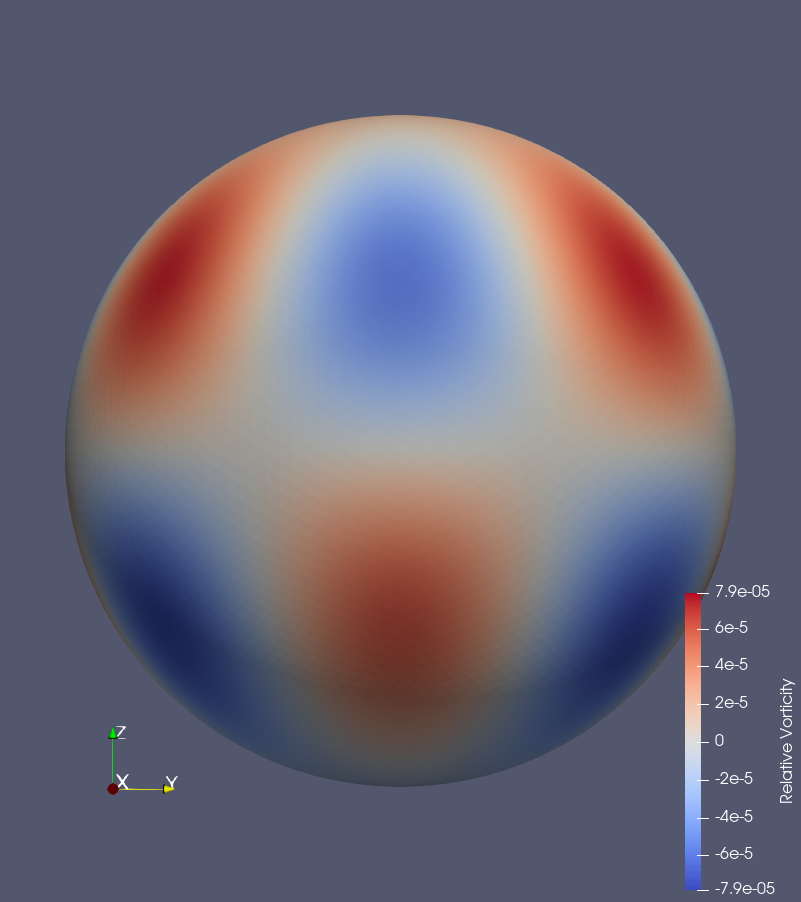
\includegraphics[scale=0.125]{Images/vorticity_0.png} &
 \hspace{-0em}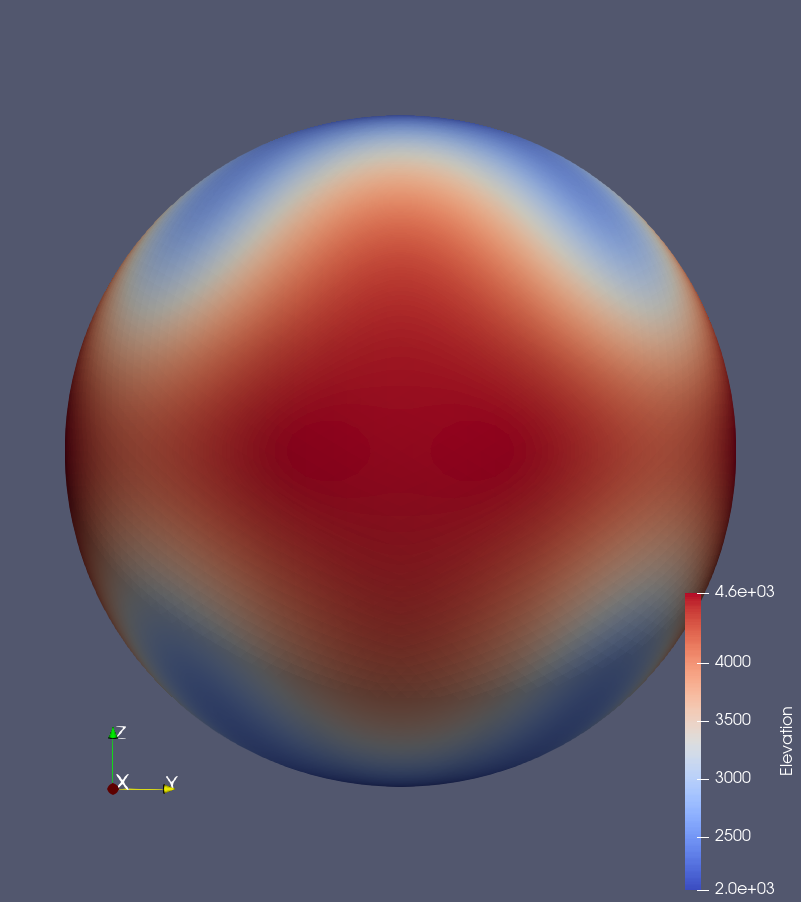
\includegraphics[scale=0.125]{Images/elevation_0.png} \\
 \hspace{-0em}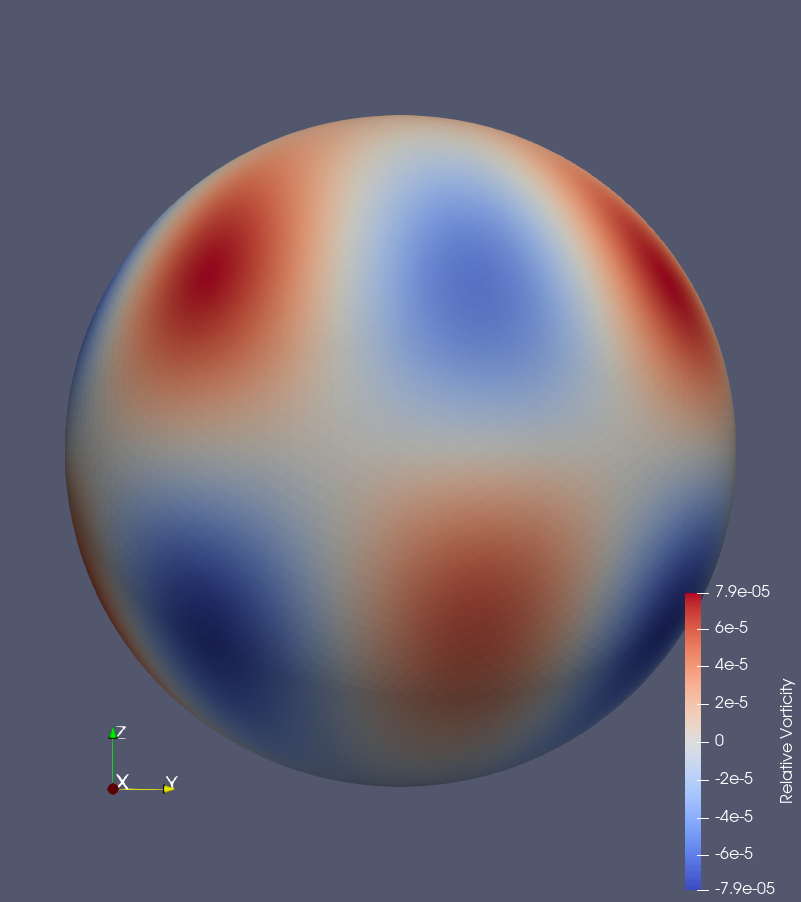
\includegraphics[scale=0.125]{Images/vorticity_24.png} &
 \hspace{-0em}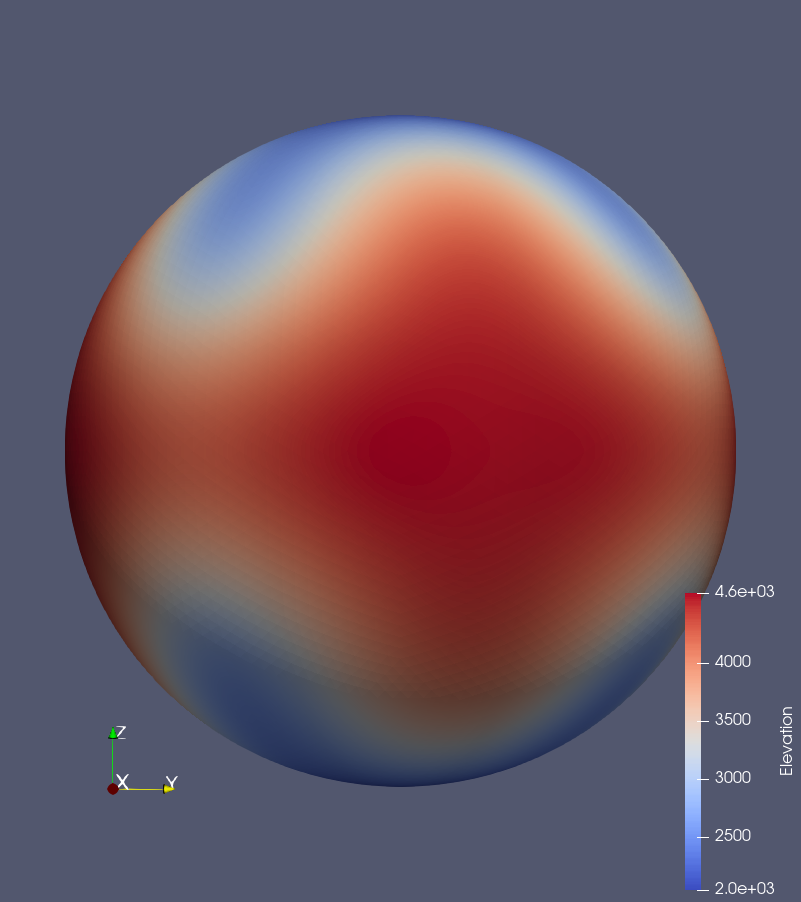
\includegraphics[scale=0.125]{Images/elevation_24.png} \\
 \end{tabular}\vspace{-10pt}
  \caption*{{\bfseries Figure 3}: TOP: initial vorticity (left) and depth (right) fields
  for Williamson test case 6. BOTTOM: fields at day 1. The shown fields are for mesh level 5.
  }
  %\label{fig1}
  \end{figure}
%  \end{minipage}\hfill
% \begin{minipage}{0.55\linewidth}
\begin{figure}[t]\centering
\begin{tabular}{c}
 \hspace{-0.4em}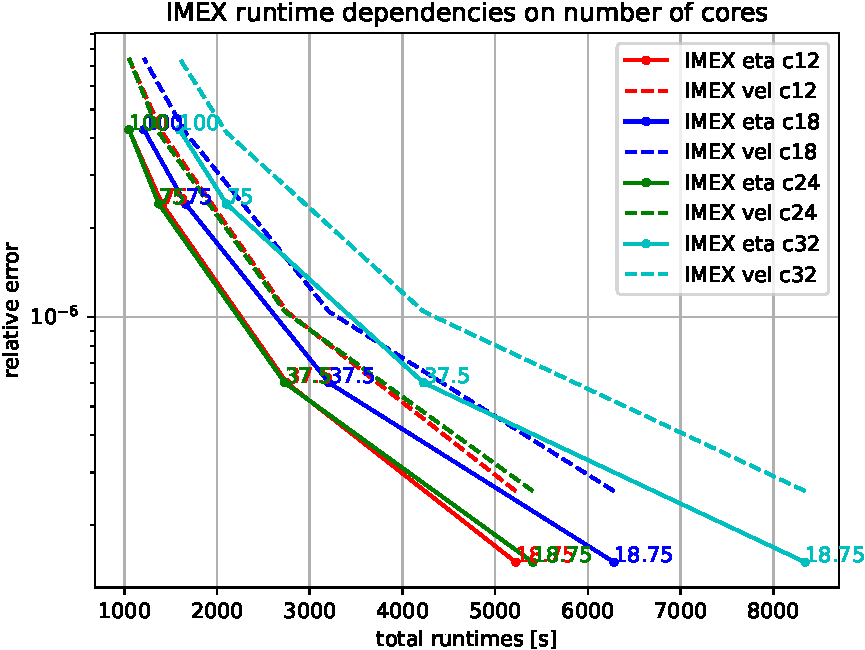
\includegraphics[scale=0.66]{Images/Figure_1_new1-crop.pdf}
  \end{tabular}
\caption*{{\bfseries Figure 4}: dependency of total runtimes
    of IMEX scheme on the number of available CPU-cores.
  }
  %\label{fig1}
  \end{figure}
  \vspace{2cm}
 % \end{minipage}


\noindent \textcolor{blue}{\textbf{Total runtimes vs. relative errors}}

  Figure 5 summarized the numerical results, i.e. total runtimes vs
  relative errors of depth $\rho$ and velocity $ u$ fields for ARK2 IMEX
  scheme, and for Gauss-Legendre (GL) schemes of order 1 (GL1), order 3 (GL2) and order 5 (GL3).

 \begin{figure}[t]\centering
 \begin{tabular}{cc}
 \hspace{-0.2em}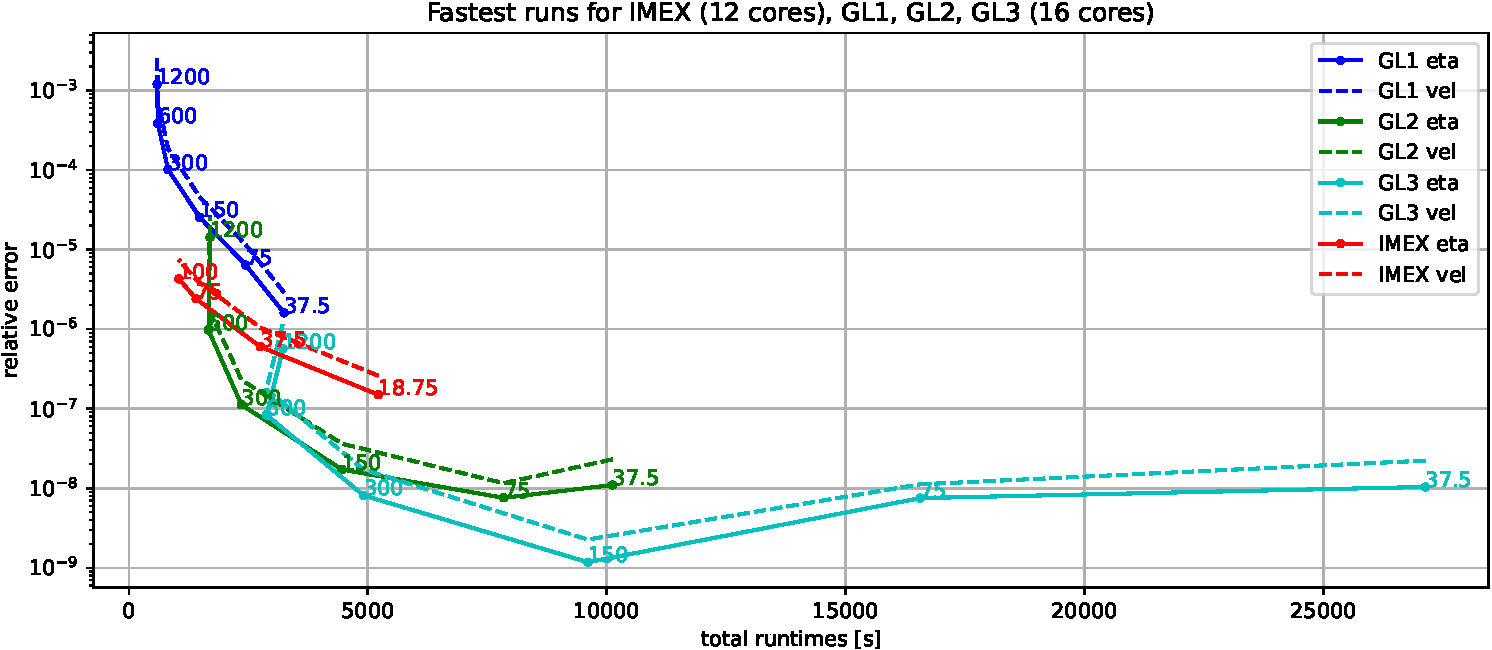
\includegraphics[scale=0.52]{Images/Figure_2_new3-crop.pdf} &
 %\hspace{-0.95em}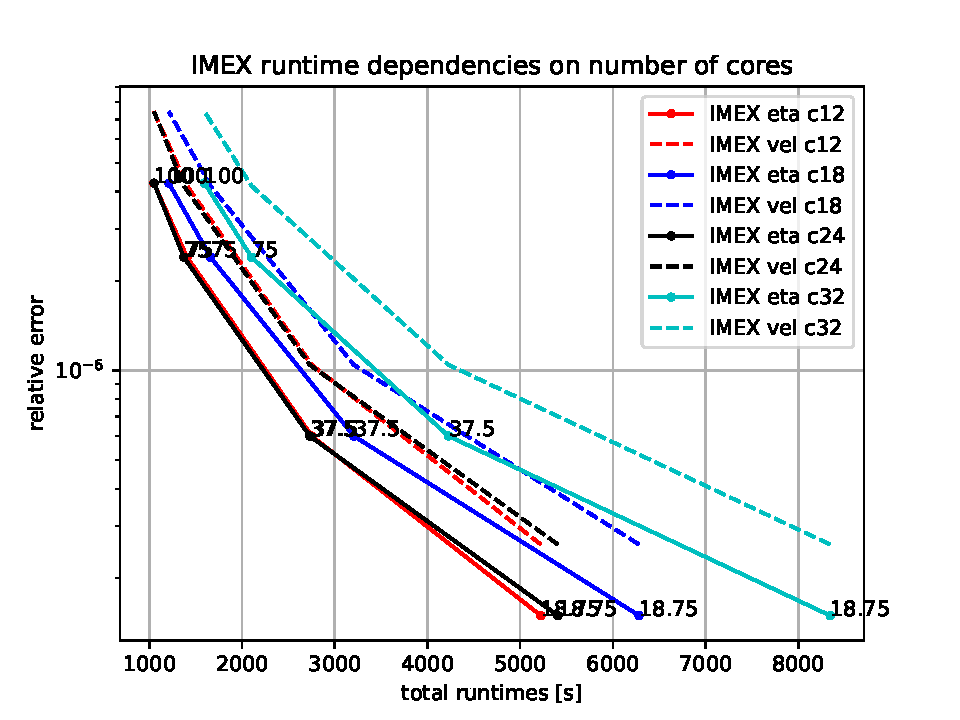
\includegraphics[scale=1.19]{Images/Figure_1_new.pdf}
  \end{tabular}\vspace{-10pt}
  \caption*{{\bfseries Figure 5}: relative errors (y-axis)
  of depth (eta) and velocity (vel) fields against the
  total runtimes of the simulations depending on the chosen schemes
  (IMEX, GL1, GL2, GL3). The total runtimes depend on the schemes,
  the time step sizes (colored figures) and on the number of available CPU-cores
  (cf. Figure 4).

  }
  \label{fig2}
  \end{figure}





 \cleardoublepage


\section{Conclusions}

   \begin{itemize}
    \item Our benchmark tests are \textbf{fair comparisons} between implicit RK schemes (of different orders) from Irksome with the ARK2 IMEX scheme, all using the same monolithic solver in Firedrake.

%    \item Figure 4 shows that under such 'fair' conditions, 3rd-order GL2 is more efficient than 2nd-order ARK2 IMEX: either it is two orders of magnitude more accurate or it requires much less runtime.
   \item Figure 5 shows that under such 'fair' conditions:\\
   (i) 3rd-order GL2 is a little slower than 2nd-order ARK2 IMEX, but about one order of magnitude more accurate; \\
   (ii) 1st order GL1 is slightly quicker but less accurate.

  \item So far, we did not explore advanced solver options, so further speedup for RK methods can be achieved.


   \item Hence, the assumption that IMEX schemes are the fastest schemes for atmosphere/ocean simulation is not necessarily correct.

   \item \textbf{Outlook:} the flexibility of Irksome in easily choosing different accuracy-orders for a vast variety of implicit RK methods allows us to further explore even more efficient time integrators.
   \end{itemize}

\bibliography{refs}

%% \begin{thebibliography}{8}
%% \bibitem{CotterShipton12} Cotter, Colin J., Jemma Shipton. "Mixed finite elements for numerical weather prediction." Journal of Computational Physics 231, no. 21 (2012): 7076-7091.

%% \bibitem{CotterShipton23}
%% \checkit{ADD PAPER DETAILS}

%% \bibitem{Farrell21} Farrell, Patrick E., Robert C. Kirby, Jorge Marchena-Menendez. "Irksome: Automating Runge-Kutta time-stepping for FE methods." ACM Transactions on Math. Software (TOMS) 47, no. 4 (2021): 1-26.

%% \bibitem{Giraldo13} Giraldo, Francis X., James F. Kelly, and Emil M. Constantinescu. "Implicit-explicit formulations of a three-dimensional nonhydrostatic unified model of the atmosphere (NUMA)." SIAM Journal on Scientific Computing 35, no. 5 (2013): B1162-B1194.
%% \end{thebibliography}






\end{document}
